\iffalse
\documentclass[journal,11pt,onecolumn]{IEEEtran}
\usepackage{setspace}
\usepackage{gensymb}
\singlespacing
\usepackage[cmex10]{amsmath}
\usepackage{amsthm}
\usepackage{mathrsfs}
\usepackage{txfonts}
\usepackage{stfloats}
\usepackage{bm}
\usepackage{cite}
\usepackage{cases}
\usepackage{subfig}
\usepackage{longtable}
\usepackage{multirow}
\usepackage{enumitem}
\usepackage{mathtools}
\usepackage{tikz}
\usepackage{circuitikz}
\usepackage{verbatim}
\usepackage[breaklinks=true]{hyperref}
\usepackage{tkz-euclide} % loads  TikZ and tkz-base
\usepackage{listings}
\usepackage{color}    
\usepackage{array}    
\usepackage{longtable}
\usepackage{calc}     
\usepackage{multirow} 
\usepackage{hhline}   
\usepackage{ifthen}   
\usepackage{lscape}     
\usepackage{chngcntr}
\usepackage{float}
\DeclareMathOperator*{\Res}{Res}
\renewcommand\thesection{\arabic{section}}
\renewcommand\thesubsection{\thesection.\arabic{subsection}}
\renewcommand\thesubsubsection{\thesubsection.\arabic{subsubsection}}

\renewcommand\thesectiondis{\arabic{section}}
\renewcommand\thesubsectiondis{\thesectiondis.\arabic{subsection}}
\renewcommand\thesubsubsectiondis{\thesubsectiondis.\arabic{subsubsection}}
\renewcommand\thetable{\arabic{table}}
% correct bad hyphenation here
\hyphenation{op-tical net-works semi-conduc-tor}
\def\inputGnumericTable{}                                 %%

\lstset{
%language=C,
frame=single, 
breaklines=true,
columns=fullflexible
}
%\lstset{
%language=tex,
%frame=single, 
%breaklines=true
%}

\title{Assignment}
\author{Barath surya M | EE22BTECH11014}
\begin{document}
\newtheorem{theorem}{Theorem}[section]
\newtheorem{problem}{Problem}
\newtheorem{proposition}{Proposition}[section]
\newtheorem{lemma}{Lemma}[section]
\newtheorem{corollary}[theorem]{Corollary}
\newtheorem{example}{Example}[section]
\newtheorem{definition}[problem]{Definition}
\newcommand{\BEQA}{\begin{eqnarray}}
\newcommand{\EEQA}{\end{eqnarray}}
\newcommand{\define}{\stackrel{\triangle}{=}}
\bibliographystyle{IEEEtran}
\providecommand{\mbf}{\mathbf}
\providecommand{\pr}[1]{\ensuremath{\Pr\left(#1\right)}}
\providecommand{\qfunc}[1]{\ensuremath{Q\left(#1\right)}}
\providecommand{\sbrak}[1]{\ensuremath{{}\left[#1\right]}}
\providecommand{\lsbrak}[1]{\ensuremath{{}\left[#1\right.}}
\providecommand{\rsbrak}[1]{\ensuremath{{}\left.#1\right]}}
\providecommand{\brak}[1]{\ensuremath{\left(#1\right)}}
\providecommand{\lbrak}[1]{\ensuremath{\left(#1\right.}}
\providecommand{\rbrak}[1]{\ensuremath{\left.#1\right)}}
\providecommand{\cbrak}[1]{\ensuremath{\left\{#1\right\}}}
\providecommand{\lcbrak}[1]{\ensuremath{\left\{#1\right.}}
\providecommand{\rcbrak}[1]{\ensuremath{\left.#1\right\}}}
\theoremstyle{remark}
\newtheorem{rem}{Remark}
\newcommand{\sgn}{\mathop{\mathrm{sgn}}}
\providecommand{\abs}[1]{\left\vert#1\right\vert}
\providecommand{\res}[1]{\Res\displaylimits_{#1}} 
\providecommand{\norm}[1]{\left\lVert#1\right\rVert}
\providecommand{\mtx}[1]{\mathbf{#1}}
\providecommand{\mean}[1]{E\left[ #1 \right]}
\providecommand{\fourier}{\overset{\mathcal{F}}{ \rightleftharpoons}}
\providecommand{\system}[1]{\overset{\mathcal{#1}}{ \longleftrightarrow}}
\newcommand{\solution}{\noindent \textbf{Solution: }}
\newcommand{\cosec}{\,\text{cosec}\,}
\providecommand{\dec}[2]{\ensuremath{\overset{#1}{\underset{#2}{\gtrless}}}}
\newcommand{\myvec}[1]{\ensuremath{\begin{pmatrix}#1\end{pmatrix}}}
\newcommand{\mydet}[1]{\ensuremath{\begin{vmatrix}#1\end{vmatrix}}}
\let\vec\mathbf
\def\putbox#1#2#3{\makebox[0in][l]{\makebox[#1][l]{}\raisebox{\baselineskip}[0in][0in]{\raisebox{#2}[0in][0in]{#3}}}}
     \def\rightbox#1{\makebox[0in][r]{#1}}
     \def\centbox#1{\makebox[0in]{#1}}
     \def\topbox#1{\raisebox{-\baselineskip}[0in][0in]{#1}}
     \def\midbox#1{\raisebox{-0.5\baselineskip}[0in][0in]{#1}}
\maketitle
\vspace{3cm}
Question 11.16.3.11\\
The accompanying venn diagram shows three events, A, B and C, and also the probabilities of the various intersections (for instance, $\pr{AB}=0.7$. Determine 
\begin{enumerate}
	\item \pr{A}
	\item \pr{BC'}
	\item \pr{A+B}
	\item \pr{AB'}
	\item \pr{BC}
	\item \text{Probability of exactly one of the three occurs}
\end{enumerate}
\begin{figure}[h!]
	\centering
	\tikzset{every picture/.style={line width=0.75pt}}   
 
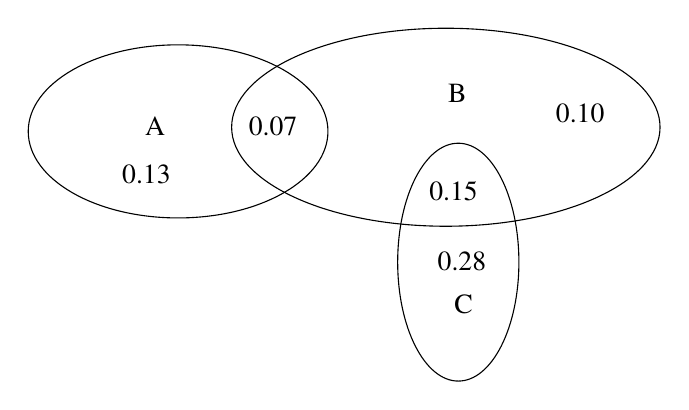
\begin{tikzpicture}[x=0.75pt,y=0.75pt,yscale=-1,xscale=1] 
 
\draw   (106,103.3) .. controls (106,80.27) and (138.33,61.6) .. (178.2,61.6) .. controls (218.07,61.6) and (250.4,80.27) .. (250.4,103.3) .. controls (250.4,126.33) and (218.07,145) .. (178.2,145) .. controls (138.33,145) and (106,126.33) .. (106,103.3) -- cycle ; 
\draw   (204,101.3) .. controls (204,74.96) and (250.2,53.6) .. (307.2,53.6) .. controls (364.2,53.6) and (410.4,74.96) .. (410.4,101.3) .. controls (410.4,127.64) and (364.2,149) .. (307.2,149) .. controls (250.2,149) and (204,127.64) .. (204,101.3) -- cycle ; 
\draw   (313.2,109) .. controls (329.33,109) and (342.4,134.65) .. (342.4,166.3) .. controls (342.4,197.95) and (329.33,223.6) .. (313.2,223.6) .. controls (297.07,223.6) and (284,197.95) .. (284,166.3) .. controls (284,134.65) and (297.07,109) .. (313.2,109) -- cycle ; 
 
\draw (161,95) node [anchor=north west][inner sep=0.75pt]   [align=left] {A}; 
\draw (307,79) node [anchor=north west][inner sep=0.75pt]   [align=left] {B}; 
\draw (310,181) node [anchor=north west][inner sep=0.75pt]   [align=left] {C}; 
\draw (150,118) node [anchor=north west][inner sep=0.75pt]   [align=left] {0.13}; 
\draw (211,95) node [anchor=north west][inner sep=0.75pt]   [align=left] {0.07}; 
\draw (298,126) node [anchor=north west][inner sep=0.75pt]   [align=left] {0.15}; 
\draw (359,89) node [anchor=north west][inner sep=0.75pt]   [align=left] {0.10}; 
\draw (302,160) node [anchor=north west][inner sep=0.75pt]   [align=left] {0.28\\}; 
 
 
\end{tikzpicture}

	\caption {generated by Latextikz}
	\label{fig:exemplar/11/16/3/11}
\end{figure}
\solution
\fi
Given:\\
From \figref{exemplar/11/16/3/11}
\begin{align}
\pr{AB}=0.07\\
\pr{AB'}=0.13\\
\pr{BC}=0.15\\
\pr{BA'C'}=0.10\\
\pr{CB'}=0.28
\end{align}
\begin{enumerate}
\item \begin{align}
	\pr{A}&= 0.13+0.07\\
	&=0.2
	\end{align}
\item \begin{align}
	\pr{BC'} &=0.07+0.10+0.15-0.15\\
	&=0.17
\end{align}
\item \begin{align}
	\pr{A+B}&= \pr{A}+\pr{B} -\pr{AB}\\
	&=0.20+\brak{0.07+0.10+0.15}-0.07\\
	&=0.45
\end{align} 
\item \begin{align}
	\pr{AB'}&=0.20-0.07\\
	&=0.13
\end{align}
\item \begin{align}
	\pr{BC}&=0.15
\end{align} 
\item \begin{align}
	\pr{\text{AB'}} +\pr{CB'}+\pr{BA'C'} &= 0.13+0.10+0.28\\
	&=0.51
\end{align} 
\end{enumerate}


 
